\documentclass[10pt]{article}
\usepackage{amsmath,amssymb}
\usepackage{longtable}
\usepackage{tikz}

\usepackage[a4paper,left=2cm,right=2cm,top=1.5cm,bottom=2cm]{geometry}
\usepackage{xcolor}
\setlength{\parindent}{0pt}
\setlength{\emergencystretch}{2em}
\begin{document}

\title{Neural Networks by Hand - Solutions}
\author{}
\date{}
\maketitle
\subsection*{Learning goals}
After this exercise, you should be able to

\begin{itemize}
\item
evaluate a simple neural network by hand,

\item
explain the role of weights, biases, and activation functions,

\item
perform a complete forward pass through a small neural network,

\item
calculate the mean squared error for a small training dataset,

\item
use backpropagation to compute gradients of the loss with respect to all trainable parameters,

\item
explain how the ReLU activation affects gradient propagation,

\item
perform one gradient-descent update,

\item
verify that a gradient step can reduce the training loss,

\item
distinguish between fitting the training points and learning the underlying function,

\item
explain why a ReLU network produces a piecewise-linear function.

\end{itemize}
The calculations in this sheet are designed to be done by hand.

\clearpage
\section*{Part I - A small neural network}
We want to approximate the function

\[
f(x)=-x^2+4x
\]

We use only the four training inputs

\[
x_i=0,\ 1,\ 2,\ 3.
\]

\subsection*{Exercise 1.1 - Generate the training data}
Evaluate the function at the four training inputs and complete the table.

\begingroup
\small
\setlength{\tabcolsep}{4pt}
\begin{longtable}{l|l}
$x_i$ & $y_i=f(x_i)$ \\[1.5pt]
\hline
\endfirsthead
$x_i$ & $y_i=f(x_i)$ \\[1.5pt]
\hline
\endhead
\rule{0pt}{2.4ex}0 &  $\phantom{-0.00}$ \\[3pt]
\rule{0pt}{2.4ex}1 &  $\phantom{-0.00}$ \\[3pt]
\rule{0pt}{2.4ex}2 &  $\phantom{-0.00}$ \\[3pt]
\rule{0pt}{2.4ex}3 &  $\phantom{-0.00}$ \\[3pt]
\end{longtable}
\endgroup
Plot the four training points and sketch the true function $f(x)=-x^2+4x$ in the range $-1\leq x\leq5$.

\begingroup\color{red}

\subsubsection*{Solution 1.1}
The training data are

\begingroup
\small
\setlength{\tabcolsep}{4pt}
\begin{longtable}{l|l}
$x_i$ & $y_i$ \\[1.5pt]
\hline
\endfirsthead
$x_i$ & $y_i$ \\[1.5pt]
\hline
\endhead
0 & 0 \\[1.5pt]
1 & 3 \\[1.5pt]
2 & 4 \\[1.5pt]
3 & 3 \\[1.5pt]
\end{longtable}
\endgroup
The function is nonlinear, so a single affine model $\hat y_i=wx_i+b$ cannot reproduce all four points exactly.

Even if a model reproduces all four training points, this does not prove that it has learned the true function between or outside those points.


The target is $f(x)=4-(x-2)^2$: a downward-opening parabola with vertex $(2,4)$ and zeros at $0$ and $4$. At the ends of the requested interval, $f(-1)=f(5)=-5$. The dots mark the training observations.
\begin{center}
\begin{tikzpicture}[x=1.45cm,y=0.48cm]
\draw[->] (-1.2,0)--(5.3,0) node[right] {$x$};
\draw[->] (0,-5.5)--(0,5.2) node[above] {$y$};
\foreach \x in {-1,1,2,3,4,5} {\draw (\x,-0.12)--(\x,0.12);\node[below] at (\x,-0.12) {\small $\x$};}
\foreach \y in {-4,-2,2,4} {\draw (-0.05,\y)--(0.05,\y);\node[left] at (-0.05,\y) {\small $\y$};}
\draw[thin,domain=-1:5,samples=81] plot (\x,{-\x*\x+4*\x});
\foreach \x/\y in {0/0,1/3,2/4,3/3} {\fill (\x,\y) circle (1.6pt);}
\end{tikzpicture}
\end{center}
\par\endgroup

\subsection*{Exercise 1.2 - Our neural network architecture}
We use the architecture

\[
1\rightarrow2\rightarrow1.
\]

There is

\begin{itemize}
\item
one input

\item
one hidden layer with two neurons

\item
one output neuron

\end{itemize}
The hidden layer uses the $ReLU$ activation

\[
\operatorname{ReLU}(z)=\max(0,z)
\]

The two hidden neurons are

\[
z_{1,i}=w_1x_i+b_1
\]

\[
h_{1,i}=\operatorname{ReLU}(z_{1,i})
\]

and

\[
z_{2,i}=w_2x_i+b_2
\]

\[
h_{2,i}=\operatorname{ReLU}(z_{2,i})
\]

The output layer is linear:

\[
\hat y_i=v_1h_{1,i}+v_2h_{2,i}+c
\]

Sketch the following

\begin{itemize}
\item
the $ReLU$ function for input values $z\in[-5,5]$

\item
the neural network

\end{itemize}
for this, count the trainable parameters first. Your drawing should contain

\begin{itemize}
\item
the input $x_i$

\item
the two hidden neurons

\item
the output $\hat y_i$

\item
all weights

\item
all biases

\item
the ReLU activation in the hidden layer

\end{itemize}
\begingroup\color{red}

\subsubsection*{Solution 1.2}
The trainable parameters are

\[
w_1,\ b_1,\ w_2,\ b_2,\ v_1,\ v_2,\ c.
\]

There are therefore 7 trainable parameters.


The ReLU graph is horizontal at zero for $z\leq0$ and follows the line $h=z$ for $z\geq0$.
\begin{center}
\begin{tikzpicture}[x=0.7cm,y=0.5cm]
\draw[->] (-5.5,0)--(5.5,0) node[right] {$z$};
\draw[->] (0,-0.5)--(0,5.6) node[above] {$\operatorname{ReLU}(z)$};
\draw[thick] (-5,0)--(0,0)--(5,5);
\node[below] at (-5,0) {$-5$};\node[below left] at (0,0) {$0$};\node[below] at (5,0) {$5$};\node[left] at (0,5) {$5$};
\end{tikzpicture}
\end{center}
The two hidden neurons apply ReLU; the output is a linear combination with bias $c$:
\begin{center}
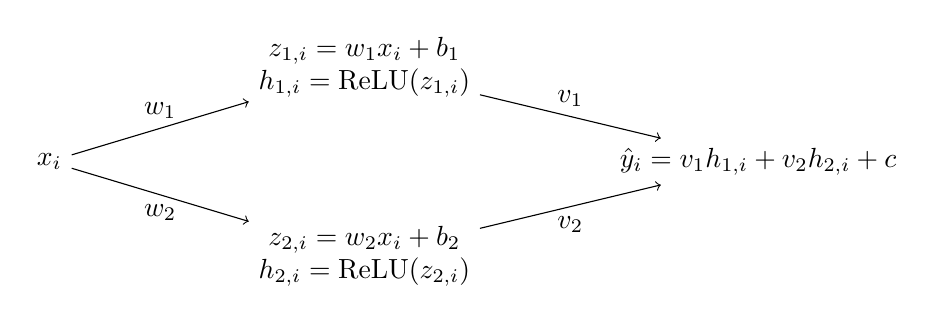
\begin{tikzpicture}[every node/.style={align=center}]
\node (x) at (0,0) {$x_i$};
\node (h1) at (4,1.2) {$z_{1,i}=w_1x_i+b_1$\\$h_{1,i}=\operatorname{ReLU}(z_{1,i})$};
\node (h2) at (4,-1.2) {$z_{2,i}=w_2x_i+b_2$\\$h_{2,i}=\operatorname{ReLU}(z_{2,i})$};
\node (y) at (9,0) {$\hat y_i=v_1h_{1,i}+v_2h_{2,i}+c$};
\draw[->] (x)--node[above] {$w_1$}(h1);\draw[->] (x)--node[below] {$w_2$}(h2);
\draw[->] (h1)--node[above] {$v_1$}(y);\draw[->] (h2)--node[below] {$v_2$}(y);
\end{tikzpicture}
\end{center}
\par\endgroup

\subsection*{Exercise 1.3 - A complete forward pass}
To build the neural network, the parameters need to be fit. We start with a list of initial guesses for which the output of the neural network is calculated. This will be compared to the training data using the mean squared error. A real neural network training proceeds until the MSE is sufficiently small. In this exercise we will however only produce a single calculation.

For the first training step, use the following initial parameters:

\[
w_1=1
\qquad
b_1=-0.5
\]

\[
w_2=-1
\qquad
b_2=2.5
\]

\[
v_1=1
\qquad
v_2=1
\qquad
c=0
\]

This exercise is divised into multiple steps:

\subsubsection*{Step 1 - Hidden-layer activations}
For each of the four training inputs, calculate

\[
z_{1,i}=w_1x_i+b_1
\]

\[
h_{1,i}=\operatorname{ReLU}(z_{1,i})
\]

and analoguous for $z_{2,i}$ and $h_{2,i}$. Complete the table below:

\begingroup
\small
\setlength{\tabcolsep}{4pt}
\begin{longtable}{l|l|l|l|l|l}
$x_i$ & $y_i$ & $z_{1,i}$ & $h_{1,i}$ & $z_{2,i}$ & $h_{2,i}$ \\[1.5pt]
\hline
\endfirsthead
$x_i$ & $y_i$ & $z_{1,i}$ & $h_{1,i}$ & $z_{2,i}$ & $h_{2,i}$ \\[1.5pt]
\hline
\endhead
\rule{0pt}{2.4ex}0 & 0 &  $\phantom{-0.00}$ &  $\phantom{-0.00}$ &  $\phantom{-0.00}$ &  $\phantom{-0.00}$ \\[3pt]
\rule{0pt}{2.4ex}1 & 3 &  $\phantom{-0.00}$ &  $\phantom{-0.00}$ &  $\phantom{-0.00}$ &  $\phantom{-0.00}$ \\[3pt]
\rule{0pt}{2.4ex}2 & 4 &  $\phantom{-0.00}$ &  $\phantom{-0.00}$ &  $\phantom{-0.00}$ &  $\phantom{-0.00}$ \\[3pt]
\rule{0pt}{2.4ex}3 & 3 &  $\phantom{-0.00}$ &  $\phantom{-0.00}$ &  $\phantom{-0.00}$ &  $\phantom{-0.00}$ \\[3pt]
\end{longtable}
\endgroup
For each hidden neuron, identify for which input values the ReLU is active.

\subsubsection*{Step 2 - Output predictions}
Using

\[
\hat y=v_1h_1+v_2h_2+c
\]

calculate the network prediction for every training point:


\begin{center}
\begingroup
\small
\setlength{\tabcolsep}{4pt}
\begin{tabular}{l|l|l|l}
$x$ & $y$ & $\hat y$ & Residual $\hat y-y$ \\ \hline
\rule{0pt}{2.4ex}0 & 0 & $\phantom{0}$ & $\phantom{0}$ \\[3pt]
\rule{0pt}{2.4ex}1 & 3 & $\phantom{0}$ & $\phantom{0}$ \\[3pt]
\rule{0pt}{2.4ex}2 & 4 & $\phantom{0}$ & $\phantom{0}$ \\[3pt]
\rule{0pt}{2.4ex}3 & 3 & $\phantom{0}$ & $\phantom{0}$ \\[3pt]
\end{tabular}
\endgroup
\end{center}


Plot the four predictions together with the four training points.

\subsubsection*{Step 3 - Calculate the loss}
We use the mean squared error

\[
L=\frac{1}{N}\sum_{i=1}^{N}(\hat y_i-y_i)^2
\]

with

\[
N=4
\]

Calculate the MSE for the current network. This is the loss before training.

\begingroup\color{red}

\subsubsection*{Solution 1.3}
Using

\[
w_1=1,\quad b_1=-0.5
\]

and

\[
w_2=-1,\quad b_2=2.5
\]

we obtain

\begingroup
\small
\setlength{\tabcolsep}{4pt}
\begin{longtable}{l|l|l|l|l|l}
$x$ & $y$ & $z_1$ & $h_1$ & $z_2$ & $h_2$ \\[1.5pt]
\hline
\endfirsthead
$x$ & $y$ & $z_1$ & $h_1$ & $z_2$ & $h_2$ \\[1.5pt]
\hline
\endhead
0 & 0 & -0.5 & 0 & 2.5 & 2.5 \\[1.5pt]
1 & 3 & 0.5 & 0.5 & 1.5 & 1.5 \\[1.5pt]
2 & 4 & 1.5 & 1.5 & 0.5 & 0.5 \\[1.5pt]
3 & 3 & 2.5 & 2.5 & -0.5 & 0 \\[1.5pt]
\end{longtable}
\endgroup
Because

\[
v_1=v_2=1,
\qquad
c=0
\]

the predictions are

\begingroup
\small
\setlength{\tabcolsep}{4pt}
\begin{longtable}{l|l|l|l|l|l}
$x$ & $y$ & $h_1$ & $h_2$ & $\hat y$ & $\hat y-y$ \\[1.5pt]
\hline
\endfirsthead
$x$ & $y$ & $h_1$ & $h_2$ & $\hat y$ & $\hat y-y$ \\[1.5pt]
\hline
\endhead
0 & 0 & 0 & 2.5 & 2.5 & 2.5 \\[1.5pt]
1 & 3 & 0.5 & 1.5 & 2.0 & -1.0 \\[1.5pt]
2 & 4 & 1.5 & 0.5 & 2.0 & -2.0 \\[1.5pt]
3 & 3 & 2.5 & 0 & 2.5 & -0.5 \\[1.5pt]
\end{longtable}
\endgroup
Thus,

\[
L=\frac{1}{4}\left(2.5^2+(-1)^2+(-2)^2+(-0.5)^2\right)
\]

so $L=2.875$


Neuron 1 is active for $x>0.5$, hence at training inputs $1,2,3$. Neuron 2 is active for $x<2.5$, hence at training inputs $0,1,2$. At the thresholds themselves the activation is zero.

In the following plot, dots are the training targets and crosses are the initial predictions.
\begin{center}
\begin{tikzpicture}[x=1.6cm,y=0.75cm]
\draw[->] (-0.3,0)--(3.5,0) node[right] {$x$};\draw[->] (0,-0.3)--(0,4.6) node[above] {$y$};
\foreach \x in {1,2,3} {\node[below] at (\x,0) {$\x$};}
\foreach \y in {1,2,3,4} {\node[left] at (0,\y) {$\y$};}
\foreach \x/\y in {0/0,1/3,2/4,3/3} {\fill (\x,\y) circle (1.6pt);}
\foreach \x/\y in {0/2.5,1/2,2/2,3/2.5} {\draw (\x-0.06,\y-0.1)--(\x+0.06,\y+0.1);\draw (\x-0.06,\y+0.1)--(\x+0.06,\y-0.1);}
\end{tikzpicture}
\end{center}
\par\endgroup

\subsection*{Exercise 1.4 - Backpropagation by hand}
We now calculate how the loss changes with respect to every trainable parameter.

The important idea is:

\[
\text{"Start at the loss and repeatedly apply the chain rule while moving backwards through the network"}
\]

We perform this calculation only once by hand. A neural-network library repeats exactly the same type of calculation automatically.

\subsubsection*{Step 1 - Start at the loss}
For one training sample the loss is

\[
L_i=(\hat y_i-y_i)^2
\]

and so the mean loss is given by a sum

\[
L=\frac{1}{4}\sum_i L_i
\]

The gradient is given by

\[
\frac{\partial L}{\partial \hat y_i}=\frac{2}{4}(\hat y_i-y_i)
\]

One defines

\[
\delta_i=\frac{\partial L}{\partial \hat y_i}
\]

Calculate $\delta_i$ for every training point.

\begingroup
\small
\setlength{\tabcolsep}{4pt}
\begin{longtable}{l|l|l|l|l}
$x_i$ & $y_i$ & $\hat y_i$ & $\hat y_i-y_i$ & $\delta=\partial L/\partial\hat y$ \\[1.5pt]
\hline
\endfirsthead
$x_i$ & $y_i$ & $\hat y_i$ & $\hat y_i-y_i$ & $\delta=\partial L/\partial\hat y$ \\[1.5pt]
\hline
\endhead
\rule{0pt}{2.4ex}0 & 0 &  $\phantom{-0.00}$ &  $\phantom{-0.00}$ &  $\phantom{-0.00}$ \\[3pt]
\rule{0pt}{2.4ex}1 & 3 &  $\phantom{-0.00}$ &  $\phantom{-0.00}$ &  $\phantom{-0.00}$ \\[3pt]
\rule{0pt}{2.4ex}2 & 4 &  $\phantom{-0.00}$ &  $\phantom{-0.00}$ &  $\phantom{-0.00}$ \\[3pt]
\rule{0pt}{2.4ex}3 & 3 &  $\phantom{-0.00}$ &  $\phantom{-0.00}$ &  $\phantom{-0.00}$ \\[3pt]
\end{longtable}
\endgroup
\subsubsection*{Step 2 - Gradients of the output layer}
\paragraph*{Gradient with respect to $v_1$}
The output is

\[
\hat y_i=v_1h_{1,i}+v_2h_{2,i}+c
\]

thus

\[
\frac{\partial \hat y_i}{\partial v_1}=h_{1,i}
\]

Use the chain rule to obtain

\[
\frac{\partial L}{\partial v_1}=\sum_i\frac{\partial L}{\partial\hat y_i}\frac{\partial\hat y_i}{\partial v_1}
\]

Therefore,

\[
\frac{\partial L}{\partial v_1}=\sum_i \delta_i h_{1,i}
\]

Calculate this gradient.

\paragraph*{Gradient with respect to $v_2$}
Analogously, calculate

\[
\frac{\partial L}{\partial v_2}=\sum_i \delta_i h_{2,i}
\]

\paragraph*{Gradient with respect to $c$}
Since

\[
\frac{\partial\hat y_i}{\partial c}=1
\]

calculate

\[
\frac{\partial L}{\partial c}=\sum_i\delta_i
\]

Record your results:

\begingroup
\small
\setlength{\tabcolsep}{4pt}
\begin{longtable}{l|l}
parameter & gradient \\[1.5pt]
\hline
\endfirsthead
parameter & gradient \\[1.5pt]
\hline
\endhead
\rule{0pt}{2.4ex}$v_1$ &  $\phantom{-0.00}$ \\[3pt]
\rule{0pt}{2.4ex}$v_2$ &  $\phantom{-0.00}$ \\[3pt]
\rule{0pt}{2.4ex}$c$ &  $\phantom{-0.00}$ \\[3pt]
\end{longtable}
\endgroup
\subsubsection*{Step 3 - Backpropagate through ReLU}
The derivative of ReLU is

\[
\operatorname{ReLU}'(z)=
\begin{cases}
0, & z<0,\\1, & z>0
\end{cases}
\]

For the values encountered in this exercise, none of the $z$ values are exactly zero.

Using your values from the forward pass, complete the table:

\begingroup
\small
\setlength{\tabcolsep}{4pt}
\begin{longtable}{l|l|l|l|l}
$x_i$ & $z_{1,i}$ & $\operatorname{ReLU}'(z_{1,i})$ & $z_{2,i}$ & $\operatorname{ReLU}'(z_{2,i})$ \\[1.5pt]
\hline
\endfirsthead
$x_i$ & $z_{1,i}$ & $\operatorname{ReLU}'(z_{1,i})$ & $z_{2,i}$ & $\operatorname{ReLU}'(z_{2,i})$ \\[1.5pt]
\hline
\endhead
\rule{0pt}{2.4ex}0 &  $\phantom{-0.00}$ &  $\phantom{-0.00}$ &  $\phantom{-0.00}$ &  $\phantom{-0.00}$ \\[3pt]
\rule{0pt}{2.4ex}1 &  $\phantom{-0.00}$ &  $\phantom{-0.00}$ &  $\phantom{-0.00}$ &  $\phantom{-0.00}$ \\[3pt]
\rule{0pt}{2.4ex}2 &  $\phantom{-0.00}$ &  $\phantom{-0.00}$ &  $\phantom{-0.00}$ &  $\phantom{-0.00}$ \\[3pt]
\rule{0pt}{2.4ex}3 &  $\phantom{-0.00}$ &  $\phantom{-0.00}$ &  $\phantom{-0.00}$ &  $\phantom{-0.00}$ \\[3pt]
\end{longtable}
\endgroup
For the first hidden neuron,

\[
\frac{\partial L}{\partial z_{1,i}}=\frac{\partial L}{\partial\hat y_i}\frac{\partial\hat y_i}{\partial h_{1,i}}\frac{\partial h_{1,i}}{\partial z_{1,i}}
\]

Because

\[
\frac{\partial\hat y_i}{\partial h_{1,i}}=v_1
\]

we obtain

\[
\frac{\partial L}{\partial z_{1,i}}=\delta_i v_1\operatorname{ReLU}'(z_{1,i})
\]

Calculate these four values.

Do the same for the second hidden neuron:

\[
\frac{\partial L}{\partial z_{2,i}}=\delta_i v_2\operatorname{ReLU}'(z_{2,i})
\]

Complete:

\begingroup
\small
\setlength{\tabcolsep}{4pt}
\begin{longtable}{l|l|l}
$x_i$ & $\partial L/\partial z_{1,i}$ & $\partial L/\partial z_{2,i}$ \\[1.5pt]
\hline
\endfirsthead
$x_i$ & $\partial L/\partial z_{1,i}$ & $\partial L/\partial z_{2,i}$ \\[1.5pt]
\hline
\endhead
\rule{0pt}{2.4ex}0 &  $\phantom{-0.00}$ &  $\phantom{-0.00}$ \\[3pt]
\rule{0pt}{2.4ex}1 &  $\phantom{-0.00}$ &  $\phantom{-0.00}$ \\[3pt]
\rule{0pt}{2.4ex}2 &  $\phantom{-0.00}$ &  $\phantom{-0.00}$ \\[3pt]
\rule{0pt}{2.4ex}3 &  $\phantom{-0.00}$ &  $\phantom{-0.00}$ \\[3pt]
\end{longtable}
\endgroup
What happens to the gradient when a ReLU neuron is inactive?

\subsubsection*{Step 4 - Gradients of the first layer}
For the first neuron,

\[
z_{1,i}=w_1x_i+b_1.
\]

Therefore,

\[
\frac{\partial z_{1,i}}{\partial w_1}=x_i
\]

and

\[
\frac{\partial z_{1,i}}{\partial b_1}=1
\]

Calculate the gradients

\[
\frac{\partial L}{\partial w_1}
\]

and

\[
\frac{\partial L}{\partial b_1}
\]

Repeat the calculation for the second hidden neuron and collect all seven gradients:

\begingroup
\small
\setlength{\tabcolsep}{4pt}
\begin{longtable}{l|l}
parameter & gradient \\[1.5pt]
\hline
\endfirsthead
parameter & gradient \\[1.5pt]
\hline
\endhead
\rule{0pt}{2.4ex}$w_1$ &  $\phantom{-0.00}$ \\[3pt]
\rule{0pt}{2.4ex}$b_1$ &  $\phantom{-0.00}$ \\[3pt]
\rule{0pt}{2.4ex}$w_2$ &  $\phantom{-0.00}$ \\[3pt]
\rule{0pt}{2.4ex}$b_2$ &  $\phantom{-0.00}$ \\[3pt]
\rule{0pt}{2.4ex}$v_1$ &  $\phantom{-0.00}$ \\[3pt]
\rule{0pt}{2.4ex}$v_2$ &  $\phantom{-0.00}$ \\[3pt]
\rule{0pt}{2.4ex}$c$ &  $\phantom{-0.00}$ \\[3pt]
\end{longtable}
\endgroup
\begingroup\color{red}

\subsubsection*{Solution 1.4}
For every sample,

\[
\delta_i=\frac{\partial L}{\partial\hat y_i}=\frac12(\hat y_i-y_i)
\]

Therefore,

\[
\delta=(1.25,-0.5,-1,-0.25)
\]

For $v_1$,

\[
\frac{\partial L}{\partial v_1}=\sum_i\delta_i h_{1,i}=1.25(0)-0.5(0.5)-1(1.5)-0.25(2.5)
\]

and therefore

\[
\frac{\partial L}{\partial v_1}
=-2.375
\]

For $v_2$,

\[
\frac{\partial L}{\partial v_2}=1.25(2.5)-0.5(1.5)-1(0.5)-0.25(0)
\]

so

\[
\frac{\partial L}{\partial v_2}
=1.875
\]

For the output bias,

\[
\frac{\partial L}{\partial c}=1.25-0.5-1-0.25=-0.5
\]

For the first hidden neuron,

\[
z_1=(-0.5,0.5,1.5,2.5),
\]

so

\[
\operatorname{ReLU}'(z_1)=(0,1,1,1)
\]

For the second hidden neuron,

\[
z_2=(2.5,1.5,0.5,-0.5)
\]

so

\[
\operatorname{ReLU}'(z_2)=(1,1,1,0)
\]

Because initially

\[
v_1=v_2=1
\]

we obtain

\[
\frac{\partial L}{\partial z_1}=(0,-0.5,-1,-0.25)
\]

and

\[
\frac{\partial L}{\partial z_2}=(1.25,-0.5,-1,0)
\]

An inactive ReLU has derivative zero, so no gradient is propagated through that neuron for that sample.

For the first hidden neuron,

\[
\frac{\partial L}{\partial w_1}=0(0)+(-0.5)(1)+(-1)(2)+(-0.25)(3)=-3.25
\]

Furthermore,

\[
\frac{\partial L}{\partial b_1}=0-0.5-1-0.25=-1.75
\]

For the second neuron,

\[
\frac{\partial L}{\partial w_2}=1.25(0)+(-0.5)(1)+(-1)(2)+0(3)=-2.5
\]

Finally,

\[
\frac{\partial L}{\partial b_2}=1.25-0.5-1=-0.25
\]

All gradients are therefore

\begingroup
\small
\setlength{\tabcolsep}{4pt}
\begin{longtable}{l|l}
parameter & gradient \\[1.5pt]
\hline
\endfirsthead
parameter & gradient \\[1.5pt]
\hline
\endhead
$w_1$ & -3.25 \\[1.5pt]
$b_1$ & -1.75 \\[1.5pt]
$w_2$ & -2.50 \\[1.5pt]
$b_2$ & -0.25 \\[1.5pt]
$v_1$ & -2.375 \\[1.5pt]
$v_2$ & 1.875 \\[1.5pt]
$c$ & -0.50 \\[1.5pt]
\end{longtable}
\endgroup


\begin{center}
\begingroup
\small
\setlength{\tabcolsep}{4pt}
\begin{tabular}{l|l|l|l|l}
$x_i$ & $y_i$ & $\hat y_i$ & $\hat y_i-y_i$ & $\delta_i$ \\ \hline
0 & 0 & 2.5 & 2.5 & 1.25 \\[1.5pt]
1 & 3 & 2 & -1 & -0.5 \\[1.5pt]
2 & 4 & 2 & -2 & -1 \\[1.5pt]
3 & 3 & 2.5 & -0.5 & -0.25 \\[1.5pt]
\end{tabular}
\endgroup
\end{center}

\begin{center}
\begingroup
\small
\setlength{\tabcolsep}{4pt}
\begin{tabular}{l|l|l|l|l|l|l}
$x_i$ & $z_{1,i}$ & $\operatorname{ReLU}^\prime(z_{1,i})$ & $z_{2,i}$ & $\operatorname{ReLU}^\prime(z_{2,i})$ & $\partial L/\partial z_{1,i}$ & $\partial L/\partial z_{2,i}$ \\ \hline
0 & -0.5 & 0 & 2.5 & 1 & 0 & 1.25 \\[1.5pt]
1 & 0.5 & 1 & 1.5 & 1 & -0.5 & -0.5 \\[1.5pt]
2 & 1.5 & 1 & 0.5 & 1 & -1 & -1 \\[1.5pt]
3 & 2.5 & 1 & -0.5 & 0 & -0.25 & 0 \\[1.5pt]
\end{tabular}
\endgroup
\end{center}
\par\endgroup

\subsection*{Exercise 1.5 - One gradient-descent step}
We now update every parameter using gradient descent. For a parameter $\theta$

\[
\theta_{\mathrm{new}}=\theta_{\mathrm{old}}-\eta\frac{\partial L}{\partial\theta}
\]

Use the learning rate

\[
\eta=0.1
\]

\subsubsection*{Step 1 - Update the parameters}
Complete the table.

\begingroup
\small
\setlength{\tabcolsep}{4pt}
\begin{longtable}{l|l|l|l}
parameter & old value & gradient & new value \\[1.5pt]
\hline
\endfirsthead
parameter & old value & gradient & new value \\[1.5pt]
\hline
\endhead
\rule{0pt}{2.4ex}$w_1$ & 1.0 &  $\phantom{-0.00}$ &  $\phantom{-0.00}$ \\[3pt]
\rule{0pt}{2.4ex}$b_1$ & -0.5 &  $\phantom{-0.00}$ &  $\phantom{-0.00}$ \\[3pt]
\rule{0pt}{2.4ex}$w_2$ & -1.0 &  $\phantom{-0.00}$ &  $\phantom{-0.00}$ \\[3pt]
\rule{0pt}{2.4ex}$b_2$ & 2.5 &  $\phantom{-0.00}$ &  $\phantom{-0.00}$ \\[3pt]
\rule{0pt}{2.4ex}$v_1$ & 1.0 &  $\phantom{-0.00}$ &  $\phantom{-0.00}$ \\[3pt]
\rule{0pt}{2.4ex}$v_2$ & 1.0 &  $\phantom{-0.00}$ &  $\phantom{-0.00}$ \\[3pt]
\rule{0pt}{2.4ex}$c$ & 0.0 &  $\phantom{-0.00}$ &  $\phantom{-0.00}$ \\[3pt]
\end{longtable}
\endgroup
\subsubsection*{Step 2 - Did training improve the model?}
Using the updated parameters, perform one more forward pass (see Exercise 1.3). (You do not need to perform another backward pass)

Calculate the new predictions and the new MSE.

\begingroup
\small
\setlength{\tabcolsep}{4pt}
\begin{longtable}{l|l|l}
$x$ & $y$ & new prediction $\hat y_{\mathrm{new}}$ \\[1.5pt]
\hline
\endfirsthead
$x$ & $y$ & new prediction $\hat y_{\mathrm{new}}$ \\[1.5pt]
\hline
\endhead
\rule{0pt}{2.4ex}0 & 0 &  $\phantom{-0.00}$ \\[3pt]
\rule{0pt}{2.4ex}1 & 3 &  $\phantom{-0.00}$ \\[3pt]
\rule{0pt}{2.4ex}2 & 4 &  $\phantom{-0.00}$ \\[3pt]
\rule{0pt}{2.4ex}3 & 3 &  $\phantom{-0.00}$ \\[3pt]
\end{longtable}
\endgroup
Compare

\[
L_{\mathrm{old}}
\]

and

\[
L_{\mathrm{new}}.
\]

Did this gradient-descent step reduce the loss? Does every single training point necessarily improve after one gradient step?

Explain why the optimizer can still reduce the total loss even if one individual prediction becomes worse.

\begingroup\color{red}

\subsubsection*{Solution 1.5}
With

\[
\eta=0.1
\]

the updated parameters are

\begingroup
\small
\setlength{\tabcolsep}{4pt}
\begin{longtable}{l|l|l|l}
parameter & old value & gradient & new value \\[1.5pt]
\hline
\endfirsthead
parameter & old value & gradient & new value \\[1.5pt]
\hline
\endhead
$w_1$ & 1.0 & -3.25 & 1.325 \\[1.5pt]
$b_1$ & -0.5 & -1.75 & -0.325 \\[1.5pt]
$w_2$ & -1.0 & -2.50 & -0.750 \\[1.5pt]
$b_2$ & 2.5 & -0.25 & 2.525 \\[1.5pt]
$v_1$ & 1.0 & -2.375 & 1.2375 \\[1.5pt]
$v_2$ & 1.0 & 1.875 & 0.8125 \\[1.5pt]
$c$ & 0.0 & -0.50 & 0.050 \\[1.5pt]
\end{longtable}
\endgroup
The new predictions are approximately

\begingroup
\small
\setlength{\tabcolsep}{4pt}
\begin{longtable}{l|l|l}
$x$ & $y$ & $\hat y_{\mathrm{new}}$ \\[1.5pt]
\hline
\endfirsthead
$x$ & $y$ & $\hat y_{\mathrm{new}}$ \\[1.5pt]
\hline
\endhead
0 & 0 & 2.102 \\[1.5pt]
1 & 3 & 2.730 \\[1.5pt]
2 & 4 & 3.760 \\[1.5pt]
3 & 3 & 4.790 \\[1.5pt]
\end{longtable}
\endgroup
The new loss is approximately

\[
L_{\mathrm{new}}\approx1.94
\]

Since

\[
1.94<2.875
\]

the gradient step has reduced the total loss.

The prediction for every individual point does not need to improve. Gradient descent follows the gradient of the combined loss over the complete dataset.


For example, at $x=3$ the updated hidden activations are $h_1=3.65$ and $h_2=0.275$, giving $\hat y_{\mathrm{new}}=4.7903125$. The error at this point grows from $-0.5$ to $1.7903125$. The reduction in the other points' squared errors outweighs this increase.

Using the unrounded predictions,
\[
L_{\mathrm{new}}=\frac{2.1015625^2+(-0.2703125)^2+(-0.24)^2+1.7903125^2}{4}=1.9381131591796875.
\]

\begin{center}
\begingroup
\small
\setlength{\tabcolsep}{4pt}
\begin{tabular}{l|l|l|l}
$x$ & $h_{1,\mathrm{new}}$ & $h_{2,\mathrm{new}}$ & $\hat y_{\mathrm{new}}$ \\ \hline
0 & 0 & 2.525 & 2.1015625 \\[1.5pt]
1 & 1 & 1.775 & 2.7296875 \\[1.5pt]
2 & 2.325 & 1.025 & 3.76 \\[1.5pt]
3 & 3.65 & 0.275 & 4.7903125 \\[1.5pt]
\end{tabular}
\endgroup
\end{center}
\par\endgroup

\clearpage
\section*{Part II - Investigating a fitted neural network}
Repeating forward pass, backpropagation, and parameter updates many times is exactly what neural-network training does.

Instead of repeating these calculations by hand, we now inspect a network whose parameters are already chosen.

Consider

\[
h_1(x)=\operatorname{ReLU}(x),
\]

\[
h_2(x)=\operatorname{ReLU}(x-1.5),
\]

and

\[
\hat f(x)=3h_1(x)-4h_2(x).
\]

This is again a network with architecture

\[
1\rightarrow2\rightarrow1.
\]

\subsection*{Exercise 2.1 - Identify the network parameters}
Write the network in the standard form

\[
z_1=w_1x+b_1,
\qquad
h_1=\operatorname{ReLU}(z_1),
\]

\[
z_2=w_2x+b_2,
\qquad
h_2=\operatorname{ReLU}(z_2),
\]

\[
\hat y=v_1h_1+v_2h_2+c.
\]

Determine the parameters

\[
w_1,\ b_1,\ w_2,\ b_2,\ v_1,\ v_2,\ c.
\]

\begingroup\color{red}

\subsubsection*{Solution 2.1}
The network is

\[
h_1=\operatorname{ReLU}(x)
\]

\[
h_2=\operatorname{ReLU}(x-1.5)
\]

\[
\hat f(x)=3h_1-4h_2
\]

Thus,

\[
w_1=1,
\qquad
b_1=0
\]

\[
w_2=1,
\qquad
b_2=-1.5
\]

\[
v_1=3,
\qquad
v_2=-4,
\qquad
c=0
\]

\par\endgroup

\subsection*{Exercise 2.2 - Check the training points}
Evaluate the fitted network at

\[
x=0,\ 1,\ 2,\ 3.
\]

Complete the table.

\begingroup
\small
\setlength{\tabcolsep}{4pt}
\begin{longtable}{l|l|l}
$x$ & true $f(x)$ & network $\hat f(x)$ \\[1.5pt]
\hline
\endfirsthead
$x$ & true $f(x)$ & network $\hat f(x)$ \\[1.5pt]
\hline
\endhead
\rule{0pt}{2.4ex}0 & 0 &  $\phantom{-0.00}$ \\[3pt]
\rule{0pt}{2.4ex}1 & 3 &  $\phantom{-0.00}$ \\[3pt]
\rule{0pt}{2.4ex}2 & 4 &  $\phantom{-0.00}$ \\[3pt]
\rule{0pt}{2.4ex}3 & 3 &  $\phantom{-0.00}$ \\[3pt]
\end{longtable}
\endgroup
Calculate the training MSE.

What is special about this result?

\begingroup\color{red}

\subsubsection*{Solution 2.2}
At the training points:

\begingroup
\small
\setlength{\tabcolsep}{4pt}
\begin{longtable}{l|l|l}
$x$ & $f(x)$ & $\hat f(x)$ \\[1.5pt]
\hline
\endfirsthead
$x$ & $f(x)$ & $\hat f(x)$ \\[1.5pt]
\hline
\endhead
0 & 0 & 0 \\[1.5pt]
1 & 3 & 3 \\[1.5pt]
2 & 4 & 4 \\[1.5pt]
3 & 3 & 3 \\[1.5pt]
\end{longtable}
\endgroup
Therefore,

\[
\mathrm{MSE}_{\mathrm{train}}=0
\]


All four training targets are reproduced exactly. This is what makes the zero training MSE special; it establishes agreement at these four inputs only.
\par\endgroup

\subsection*{Exercise 2.3 - Has the network learned the true function?}
Now evaluate both the true function and the neural network at new input values:

\[
x=0.5,\ 1.5,\ 2.5,\ 4.
\]

Complete the table.

\begingroup
\small
\setlength{\tabcolsep}{4pt}
\begin{longtable}{l|l|l|l}
$x$ & true $f(x)$ & network $\hat f(x)$ & difference \\[1.5pt]
\hline
\endfirsthead
$x$ & true $f(x)$ & network $\hat f(x)$ & difference \\[1.5pt]
\hline
\endhead
\rule{0pt}{2.4ex}0.5 &  $\phantom{-0.00}$ &  $\phantom{-0.00}$ &  $\phantom{-0.00}$ \\[3pt]
\rule{0pt}{2.4ex}1.5 &  $\phantom{-0.00}$ &  $\phantom{-0.00}$ &  $\phantom{-0.00}$ \\[3pt]
\rule{0pt}{2.4ex}2.5 &  $\phantom{-0.00}$ &  $\phantom{-0.00}$ &  $\phantom{-0.00}$ \\[3pt]
\rule{0pt}{2.4ex}4.0 &  $\phantom{-0.00}$ &  $\phantom{-0.00}$ &  $\phantom{-0.00}$ \\[3pt]
\end{longtable}
\endgroup
Discuss:

\begin{enumerate}
\item
The network has zero training error. Has it learned the exact function?

\item
Why is performance on unseen inputs important?

\end{enumerate}
\begingroup\color{red}

\subsubsection*{Solution 2.3}
However, at new inputs:

\begingroup
\small
\setlength{\tabcolsep}{4pt}
\begin{longtable}{l|l|l|l}
$x$ & true $f(x)$ & network $\hat f(x)$ & difference $\hat f-f$ \\[1.5pt]
\hline
\endfirsthead
$x$ & true $f(x)$ & network $\hat f(x)$ & difference $\hat f-f$ \\[1.5pt]
\hline
\endhead
0.5 & 1.75 & 1.50 & -0.25 \\[1.5pt]
1.5 & 3.75 & 4.50 & 0.75 \\[1.5pt]
2.5 & 3.75 & 3.50 & -0.25 \\[1.5pt]
4.0 & 0.00 & 2.00 & 2.00 \\[1.5pt]
\end{longtable}
\endgroup
Thus, zero training error does not imply that the exact underlying function has been learned.


Evaluation on unseen inputs checks whether the fitted relationship also predicts observations that were not used to choose the parameters. The discrepancies in the table show that the exact quadratic function has not been recovered.
\par\endgroup

\subsection*{Exercise 2.4 - What function has the ReLU network learned?}
The fitted network is

\[
\hat f(x)=3\operatorname{ReLU}(x)-4\operatorname{ReLU}(x-1.5)
\]

Because ReLU changes its behavior at zero, the expression changes at

\[
x=0
\]

and

\[
x=1.5
\]

Consider the three regions separately and determine $\hat f(x)$. Write the final result as

\[
\hat f(x)=
\begin{cases}
\ldots, & x<0,\\
\ldots, & 0\leq x<1.5,\\
\ldots, & x\geq1.5
\end{cases}
\]

Plot the function. What is the most important visual difference between the quadratic target function and the ReLU network?

\begingroup\color{red}

\subsubsection*{Solution 2.4}
For

\[
x<0
\]

both ReLUs are zero, so

\[
\hat f(x)=0
\]

For

\[
0\leq x<1.5
\]

we have

\[
\operatorname{ReLU}(x)=x
\]

and

\[
\operatorname{ReLU}(x-1.5)=0
\]

Therefore,

\[
\hat f(x)=3x
\]

For

\[
x\geq1.5
\]

both ReLUs are active:

\[
\hat f(x)=3x-4(x-1.5)
\]

Thus,

\[
\hat f(x)=3x-4x+6=6-x
\]

The complete function is

\[
\hat f(x)=
\begin{cases}
0, & x<0,\\
3x, & 0\leq x<1.5,\\
6-x, & x\geq1.5
\end{cases}
\]

The true function is quadratic, while the ReLU network is piecewise linear.

The locations of the changes in slope are determined by the points at which the pre-activations of the hidden ReLU neurons cross zero.

Additional hidden ReLU neurons can introduce additional changes in slope and therefore allow a finer piecewise-linear approximation.


The solid curve is the target; the dashed line is the fitted shallow network. Both pass through the training points.
\begin{center}
\begin{tikzpicture}[x=1.45cm,y=0.48cm]
\draw[->] (-1.2,0)--(5.3,0) node[right] {$x$};
\draw[->] (0,-5.5)--(0,5.2) node[above] {$y$};
\foreach \x in {-1,1,2,3,4,5} {\draw (\x,-0.12)--(\x,0.12);\node[below] at (\x,-0.12) {\small $\x$};}
\foreach \y in {-4,-2,2,4} {\draw (-0.05,\y)--(0.05,\y);\node[left] at (-0.05,\y) {\small $\y$};}
\draw[thin,domain=-1:5,samples=81] plot (\x,{-\x*\x+4*\x});
\foreach \x/\y in {0/0,1/3,2/4,3/3} {\fill (\x,\y) circle (1.6pt);}
\draw[thick,dashed] plot coordinates {(-1,0) (0,0) (1.5,4.5) (5,1)};
\end{tikzpicture}
\end{center}
\par\endgroup

\clearpage
\section*{Part III - A deeper neural network}
So far, we have considered a neural network with one hidden layer. We now investigate a deeper network with the architecture

\[
1\rightarrow3\rightarrow3\rightarrow1
\]

There is

\begin{itemize}
\item
one input

\item
a first hidden layer with three neurons

\item
a second hidden layer with three neurons

\item
one output neuron

\end{itemize}
Both hidden layers use the $ReLU$ activation function.

In this part, the parameters are already given. You do not need to perform backpropagation for this larger network. The goal is to understand how information is propagated through multiple hidden layers and how additional neurons can change the shape of the learned function.

\subsection*{Exercise 3.1 - Architecture and number of parameters}
For a fully connected neural network, every neuron in one layer is connected to every neuron in the next layer.

\begin{enumerate}
\item
Draw the architecture

\end{enumerate}
\[
1\rightarrow3\rightarrow3\rightarrow1
\]

\begin{enumerate}
\setcounter{enumi}{1}
\item
Count the number of weights and biases between the input and the first hidden layer.

\item
Count the number of weights and biases between the first and second hidden layers.

\item
Count the number of weights and biases between the second hidden layer and the output.

\item
Determine the total number of trainable parameters.

\end{enumerate}
Compare this number with the seven trainable parameters of the network from Parts I and II.

\begingroup\color{red}

\subsubsection*{Solution 3.1}
For the architecture

\[
1\rightarrow3\rightarrow3\rightarrow1
\]

the number of parameters can be counted layer by layer. Between the input and the first hidden layer there are

\[
1\cdot3=3
\]

weights and 3 biases. This gives

\[
3+3=6
\]

parameters.

Between the first and second hidden layers there are

\[
3\cdot3=9
\]

weights and 3 biases. This gives

\[
9+3=12
\]

parameters.

Between the second hidden layer and the output there are

\[
3\cdot1=3
\]

weights and 1 bias. This gives

\[
3+1=4
\]

parameters.

Thus, the complete network contains

\[
6+12+4=22
\]

trainable parameters.

The smaller network from Parts I and II contains only 7 trainable parameters. The deeper network therefore has considerably more degrees of freedom.


The diagram shows every connection of the fully connected architecture. Each hidden neuron and the output also have their own bias. Zero-valued weights in the specified example still belong to the 22 parameters of this architecture.
\begin{center}
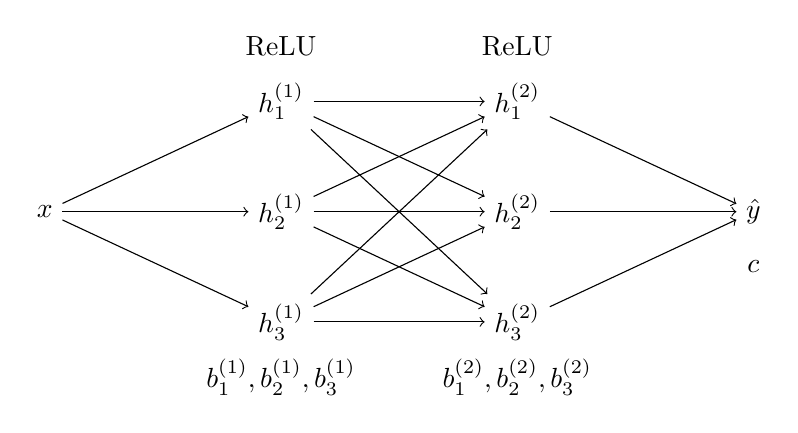
\begin{tikzpicture}
\node (x) at (0,0) {$x$};\node (y) at (9,0) {$\hat y$};
\foreach \i/\v in {1/1.4,2/0,3/-1.4} {
\node (a\i) at (3,\v) {$h^{(1)}_\i$};\node (b\i) at (6,\v) {$h^{(2)}_\i$};
\draw[->] (x)--(a\i);\draw[->] (b\i)--(y);}
\foreach \i in {1,2,3} {\foreach \j in {1,2,3} {\draw[->] (a\i)--(b\j);}}
\node at (3,2.1) {ReLU};\node at (6,2.1) {ReLU};
\node at (3,-2.1) {$b^{(1)}_1,b^{(1)}_2,b^{(1)}_3$};\node at (6,-2.1) {$b^{(2)}_1,b^{(2)}_2,b^{(2)}_3$};\node at (9,-0.7) {$c$};
\end{tikzpicture}
\end{center}
\par\endgroup

\subsection*{Exercise 3.2 - First hidden layer}
The first hidden layer is defined by

\[
z^{(1)}_{1,i}=x_i,
\qquad
h^{(1)}_{1,i}=\operatorname{ReLU}(z^{(1)}_{1,i}),
\]

\[
z^{(1)}_{2,i}=x_i-1,
\qquad
h^{(1)}_{2,i}=\operatorname{ReLU}(z^{(1)}_{2,i}),
\]

and

\[
z^{(1)}_{3,i}=x_i-2,
\qquad
h^{(1)}_{3,i}=\operatorname{ReLU}(z^{(1)}_{3,i}).
\]

Calculate the activations for the four training inputs.

\begingroup
\small
\setlength{\tabcolsep}{4pt}
\begin{longtable}{l|l|l|l|l|l|l}
$x_i$ & $z^{(1)}_{1,i}$ & $h^{(1)}_{1,i}$ & $z^{(1)}_{2,i}$ & $h^{(1)}_{2,i}$ & $z^{(1)}_{3,i}$ & $h^{(1)}_{3,i}$ \\[1.5pt]
\hline
\endfirsthead
$x_i$ & $z^{(1)}_{1,i}$ & $h^{(1)}_{1,i}$ & $z^{(1)}_{2,i}$ & $h^{(1)}_{2,i}$ & $z^{(1)}_{3,i}$ & $h^{(1)}_{3,i}$ \\[1.5pt]
\hline
\endhead
\rule{0pt}{2.4ex}0 &  $\phantom{-0.00}$ &  $\phantom{-0.00}$ &  $\phantom{-0.00}$ &  $\phantom{-0.00}$ &  $\phantom{-0.00}$ &  $\phantom{-0.00}$ \\[3pt]
\rule{0pt}{2.4ex}1 &  $\phantom{-0.00}$ &  $\phantom{-0.00}$ &  $\phantom{-0.00}$ &  $\phantom{-0.00}$ &  $\phantom{-0.00}$ &  $\phantom{-0.00}$ \\[3pt]
\rule{0pt}{2.4ex}2 &  $\phantom{-0.00}$ &  $\phantom{-0.00}$ &  $\phantom{-0.00}$ &  $\phantom{-0.00}$ &  $\phantom{-0.00}$ &  $\phantom{-0.00}$ \\[3pt]
\rule{0pt}{2.4ex}3 &  $\phantom{-0.00}$ &  $\phantom{-0.00}$ &  $\phantom{-0.00}$ &  $\phantom{-0.00}$ &  $\phantom{-0.00}$ &  $\phantom{-0.00}$ \\[3pt]
\end{longtable}
\endgroup
At which input value does each of the three neurons become active?

How does this differ from the two-neuron hidden layer considered previously?

\begingroup\color{red}

\subsubsection*{Solution 3.2}
The first hidden layer is

\[
h^{(1)}_1=\operatorname{ReLU}(x)
\]

\[
h^{(1)}_2=\operatorname{ReLU}(x-1)
\]

and

\[
h^{(1)}_3=\operatorname{ReLU}(x-2)
\]

For the four training points:

\begingroup
\small
\setlength{\tabcolsep}{4pt}
\begin{longtable}{l|l|l|l|l|l|l}
$x_i$ & $z^{(1)}_{1,i}$ & $h^{(1)}_{1,i}$ & $z^{(1)}_{2,i}$ & $h^{(1)}_{2,i}$ & $z^{(1)}_{3,i}$ & $h^{(1)}_{3,i}$ \\[1.5pt]
\hline
\endfirsthead
$x_i$ & $z^{(1)}_{1,i}$ & $h^{(1)}_{1,i}$ & $z^{(1)}_{2,i}$ & $h^{(1)}_{2,i}$ & $z^{(1)}_{3,i}$ & $h^{(1)}_{3,i}$ \\[1.5pt]
\hline
\endhead
0 & 0 & 0 & -1 & 0 & -2 & 0 \\[1.5pt]
1 & 1 & 1 & 0 & 0 & -1 & 0 \\[1.5pt]
2 & 2 & 2 & 1 & 1 & 0 & 0 \\[1.5pt]
3 & 3 & 3 & 2 & 2 & 1 & 1 \\[1.5pt]
\end{longtable}
\endgroup
The three neurons change their behavior at

\[
x=0,\qquad x=1,\qquad x=2
\]

Thus, the first hidden layer introduces three different ReLU thresholds.

Compared with the previous two-neuron hidden layer, more hidden neurons allow the network to create more distinct regions in which the overall slope may change.


The activation conditions are $x>0$, $x>1$ and $x>2$, respectively; at the threshold each activation is still zero. Among the training inputs, the active sets are $\{1,2,3\}$, $\{2,3\}$ and $\{3\}$. The fitted two-neuron network in Part II has thresholds $0$ and $1.5$; the initial network in Part I has thresholds $0.5$ and $2.5$, with the second neuron active to the left of $2.5$.
\par\endgroup

\subsection*{Exercise 3.3 - Second hidden layer}
The second hidden layer receives the three outputs of the first hidden layer as its inputs.

It is defined by

\[
z^{(2)}_{1,i}=h^{(1)}_{1,i},
\qquad
h^{(2)}_{1,i}=\operatorname{ReLU}(z^{(2)}_{1,i})
\]

\[
z^{(2)}_{2,i}=h^{(1)}_{1,i}-h^{(1)}_{2,i},
\qquad
h^{(2)}_{2,i}=\operatorname{ReLU}(z^{(2)}_{2,i})
\]

and

\[
z^{(2)}_{3,i}=h^{(1)}_{2,i}-h^{(1)}_{3,i},
\qquad
h^{(2)}_{3,i}=\operatorname{ReLU}(z^{(2)}_{3,i})
\]

Use the results from Exercise 3.2 and complete the table.

\begingroup
\small
\setlength{\tabcolsep}{4pt}
\begin{longtable}{l|l|l|l|l|l|l}
$x$ & $z^{(2)}_{1,i}$ & $h^{(2)}_{1,i}$ & $z^{(2)}_{2,i}$ & $h^{(2)}_{2,i}$ & $z^{(2)}_{3,i}$ & $h^{(2)}_{3,i}$ \\[1.5pt]
\hline
\endfirsthead
$x$ & $z^{(2)}_{1,i}$ & $h^{(2)}_{1,i}$ & $z^{(2)}_{2,i}$ & $h^{(2)}_{2,i}$ & $z^{(2)}_{3,i}$ & $h^{(2)}_{3,i}$ \\[1.5pt]
\hline
\endhead
\rule{0pt}{2.4ex}0 &  $\phantom{-0.00}$ &  $\phantom{-0.00}$ &  $\phantom{-0.00}$ &  $\phantom{-0.00}$ &  $\phantom{-0.00}$ &  $\phantom{-0.00}$ \\[3pt]
\rule{0pt}{2.4ex}1 &  $\phantom{-0.00}$ &  $\phantom{-0.00}$ &  $\phantom{-0.00}$ &  $\phantom{-0.00}$ &  $\phantom{-0.00}$ &  $\phantom{-0.00}$ \\[3pt]
\rule{0pt}{2.4ex}2 &  $\phantom{-0.00}$ &  $\phantom{-0.00}$ &  $\phantom{-0.00}$ &  $\phantom{-0.00}$ &  $\phantom{-0.00}$ &  $\phantom{-0.00}$ \\[3pt]
\rule{0pt}{2.4ex}3 &  $\phantom{-0.00}$ &  $\phantom{-0.00}$ &  $\phantom{-0.00}$ &  $\phantom{-0.00}$ &  $\phantom{-0.00}$ &  $\phantom{-0.00}$ \\[3pt]
\end{longtable}
\endgroup
Notice that the second hidden layer no longer acts directly on $x$. It transforms features that were already created by the first hidden layer.

\begingroup\color{red}

\subsubsection*{Solution 3.3}
The second hidden layer is defined by

\[
h^{(2)}_1=\operatorname{ReLU}\left(h^{(1)}_1\right)
\]

\[
h^{(2)}_2=\operatorname{ReLU}\left(h^{(1)}_1-h^{(1)}_2\right)
\]

and

\[
h^{(2)}_3=\operatorname{ReLU}\left(h^{(1)}_2-h^{(1)}_3\right)
\]

Using the results from the first hidden layer gives

\begingroup
\small
\setlength{\tabcolsep}{4pt}
\begin{longtable}{l|l|l|l|l|l|l}
$x_i$ & $z^{(2)}_{1,i}$ & $h^{(2)}_{1,i}$ & $z^{(2)}_{2,i}$ & $h^{(2)}_{2,i}$ & $z^{(2)}_{3,i}$ & $h^{(2)}_{3,i}$ \\[1.5pt]
\hline
\endfirsthead
$x_i$ & $z^{(2)}_{1,i}$ & $h^{(2)}_{1,i}$ & $z^{(2)}_{2,i}$ & $h^{(2)}_{2,i}$ & $z^{(2)}_{3,i}$ & $h^{(2)}_{3,i}$ \\[1.5pt]
\hline
\endhead
0 & 0 & 0 & 0 & 0 & 0 & 0 \\[1.5pt]
1 & 1 & 1 & 1 & 1 & 0 & 0 \\[1.5pt]
2 & 2 & 2 & 1 & 1 & 1 & 1 \\[1.5pt]
3 & 3 & 3 & 1 & 1 & 1 & 1 \\[1.5pt]
\end{longtable}
\endgroup
The important difference from the first hidden layer is that these neurons no longer receive the original input $x$ directly.

Instead, they receive the features

\[
h^{(1)}_1,\qquad h^{(1)}_2,\qquad h^{(1)}_3
\]

that were constructed by the previous layer.

The second hidden layer therefore combines already transformed information.

\par\endgroup

\subsection*{Exercise 3.4 - Output of the deep network}
The output layer is

\[
\hat f_{\mathrm{deep}}(x)=-h^{(2)}_1+4h^{(2)}_2+2h^{(2)}_3.
\]

Calculate the prediction for every training point.

\begingroup
\small
\setlength{\tabcolsep}{4pt}
\begin{longtable}{l|l|l}
$x_i$ & true $f(x_i)$ & deep network $\hat f_{\mathrm{deep}}(x_i)$ \\[1.5pt]
\hline
\endfirsthead
$x_i$ & true $f(x_i)$ & deep network $\hat f_{\mathrm{deep}}(x_i)$ \\[1.5pt]
\hline
\endhead
\rule{0pt}{2.4ex}0 & 0 &  $\phantom{-0.00}$ \\[3pt]
\rule{0pt}{2.4ex}1 & 3 &  $\phantom{-0.00}$ \\[3pt]
\rule{0pt}{2.4ex}2 & 4 &  $\phantom{-0.00}$ \\[3pt]
\rule{0pt}{2.4ex}3 & 3 &  $\phantom{-0.00}$ \\[3pt]
\end{longtable}
\endgroup
Calculate the training MSE.

Compare the result with the fitted $1\rightarrow2\rightarrow1$ network from Part II.

\begin{itemize}
\item
Do both networks achieve the same training error?

\item
Does this imply that both networks represent the same function?

\end{itemize}
\begingroup\color{red}

\subsubsection*{Solution 3.4}
The output is

\[
\hat f_{\mathrm{deep}}(x)=-h^{(2)}_1+4h^{(2)}_2+2h^{(2)}_3
\]

Using the activations from Exercise 3.3:

\begingroup
\small
\setlength{\tabcolsep}{4pt}
\begin{longtable}{l|l|l|l|l|l}
$x_i$ & true $f(x_i)$ & $h^{(2)}_1$ & $h^{(2)}_2$ & $h^{(2)}_3$ & \shortstack[l]{deep network \\ $\hat f_{\mathrm{deep}}(x_i)$} \\[1.5pt]
\hline
\endfirsthead
$x_i$ & true $f(x_i)$ & $h^{(2)}_1$ & $h^{(2)}_2$ & $h^{(2)}_3$ & \shortstack[l]{deep network \\ $\hat f_{\mathrm{deep}}(x_i)$} \\[1.5pt]
\hline
\endhead
0 & 0 & 0 & 0 & 0 & 0 \\[1.5pt]
1 & 3 & 1 & 1 & 0 & 3 \\[1.5pt]
2 & 4 & 2 & 1 & 1 & 4 \\[1.5pt]
3 & 3 & 3 & 1 & 1 & 3 \\[1.5pt]
\end{longtable}
\endgroup
Thus, the training MSE is

\[
\mathrm{MSE}_{\mathrm{train}}=0
\]

The shallow network from Part II also has zero training error.

However, this does not imply that both networks represent the same function. The training loss only compares the predictions at the four training points. The networks may behave differently between or outside these points.

\par\endgroup

\subsection*{Exercise 3.5 - Test the network between the training points}
The two networks both reproduce the four training points exactly. We now compare what they predict between the training points.

Evaluate

\[
f(x)=-x^2+4x
\]

at

\[
x=0.5,\ 1.25,\ 1.75,\ 2.5
\]

and use your result from the shallow network of Part II. For the deep network, perform the forward pass through both hidden layers and complete the table.

\begingroup
\small
\setlength{\tabcolsep}{4pt}
\begin{longtable}{l|l|l|l}
$x_i$ & true $f(x_i)$ & shallow network & deep network \\[1.5pt]
\hline
\endfirsthead
$x_i$ & true $f(x_i)$ & shallow network & deep network \\[1.5pt]
\hline
\endhead
\rule{0pt}{2.4ex}0.5 &  $\phantom{-0.00}$ &  $\phantom{-0.00}$ &  $\phantom{-0.00}$ \\[3pt]
\rule{0pt}{2.4ex}1.25 &  $\phantom{-0.00}$ &  $\phantom{-0.00}$ &  $\phantom{-0.00}$ \\[3pt]
\rule{0pt}{2.4ex}1.75 &  $\phantom{-0.00}$ &  $\phantom{-0.00}$ &  $\phantom{-0.00}$ \\[3pt]
\rule{0pt}{2.4ex}2.5 &  $\phantom{-0.00}$ &  $\phantom{-0.00}$ &  $\phantom{-0.00}$ \\[3pt]
\end{longtable}
\endgroup
Which network is closer to the true function at these points? Why can two networks with zero training error behave differently between the training observations?

\begingroup\color{red}

\subsubsection*{Solution 3.5}
The true target function is

\[
f(x)=-x^2+4x
\]

The true values are

\[
f(0.5)=1.75
\]

\[
f(1.25)=3.4375
\]

\[
f(1.75)=3.9375
\]

and

\[
f(2.5)=3.75
\]

For the shallow network,

\[
\hat f_{\mathrm{shallow}}(x)=
\begin{cases}
0, & x<0,\\
3x, & 0\leq x<1.5,\\
6-x, & x\geq1.5
\end{cases}
\]

Therefore,

\[
\hat f_{\mathrm{shallow}}(0.5)=1.5
\]

\[
\hat f_{\mathrm{shallow}}(1.25)=3.75
\]

\[
\hat f_{\mathrm{shallow}}(1.75)=4.25
\]

and

\[
\hat f_{\mathrm{shallow}}(2.5)=3.5
\]

For the deeper network, the forward pass gives

\[
\hat f_{\mathrm{deep}}(0.5)=1.5
\]

\[
\hat f_{\mathrm{deep}}(1.25)=3.25
\]

\[
\hat f_{\mathrm{deep}}(1.75)=3.75
\]

and

\[
\hat f_{\mathrm{deep}}(2.5)=3.5
\]

The comparison is therefore

\begingroup
\small
\setlength{\tabcolsep}{4pt}
\begin{longtable}{l|l|l|l}
$x_i$ & true $f(x_i)$ & shallow network & deep network \\[1.5pt]
\hline
\endfirsthead
$x_i$ & true $f(x_i)$ & shallow network & deep network \\[1.5pt]
\hline
\endhead
0.5 & 1.7500 & 1.5000 & 1.5000 \\[1.5pt]
1.25 & 3.4375 & 3.7500 & 3.2500 \\[1.5pt]
1.75 & 3.9375 & 4.2500 & 3.7500 \\[1.5pt]
2.5 & 3.7500 & 3.5000 & 3.5000 \\[1.5pt]
\end{longtable}
\endgroup
At $x=0.5$ and $x=2.5$, both networks have the same error.

At $x=1.25$ and $x=1.75$, the deeper network is closer to the true quadratic function.

Thus, both networks have zero training error, but they interpolate the training observations differently.


The forward passes through both hidden layers are:

\begin{center}
\begingroup
\small
\setlength{\tabcolsep}{4pt}
\begin{tabular}{l|l|l|l|l|l|l}
$x$ & $z^{(1)}_1$ & $h^{(1)}_1$ & $z^{(1)}_2$ & $h^{(1)}_2$ & $z^{(1)}_3$ & $h^{(1)}_3$ \\ \hline
0.5 & 0.5 & 0.5 & -0.5 & 0 & -1.5 & 0 \\[1.5pt]
1.25 & 1.25 & 1.25 & 0.25 & 0.25 & -0.75 & 0 \\[1.5pt]
1.75 & 1.75 & 1.75 & 0.75 & 0.75 & -0.25 & 0 \\[1.5pt]
2.5 & 2.5 & 2.5 & 1.5 & 1.5 & 0.5 & 0.5 \\[1.5pt]
\end{tabular}
\endgroup
\end{center}

\begin{center}
\begingroup
\small
\setlength{\tabcolsep}{4pt}
\begin{tabular}{l|l|l|l|l|l|l}
$x$ & $z^{(2)}_1$ & $h^{(2)}_1$ & $z^{(2)}_2$ & $h^{(2)}_2$ & $z^{(2)}_3$ & $h^{(2)}_3$ \\ \hline
0.5 & 0.5 & 0.5 & 0.5 & 0.5 & 0 & 0 \\[1.5pt]
1.25 & 1.25 & 1.25 & 1.0 & 1.0 & 0.25 & 0.25 \\[1.5pt]
1.75 & 1.75 & 1.75 & 1.0 & 1.0 & 0.75 & 0.75 \\[1.5pt]
2.5 & 2.5 & 2.5 & 1.0 & 1.0 & 1.0 & 1.0 \\[1.5pt]
\end{tabular}
\endgroup
\end{center}
The absolute errors at $x=0.5,1.25,1.75,2.5$ are $(0.25,0.3125,0.3125,0.25)$ for the shallow network and $(0.25,0.1875,0.1875,0.25)$ for the deep network. Agreement at finitely many training points leaves the functions between those points undetermined.
\par\endgroup

\subsection*{Exercise 3.6 - What function has the deeper network learned?}
Determine the output of the deeper network in the following regions:

\begin{enumerate}
\item
$x<0$

\item
$0\leq x<1$

\item
$1\leq x<2$

\item
$x\geq2$

\end{enumerate}
Write the result as a piecewise function

\[
\hat f_{\mathrm{deep}}(x)=
\begin{cases}
\ldots, & x<0,\\
\ldots, & 0\leq x<1,\\
\ldots, & 1\leq x<2,\\
\ldots, & x\geq2
\end{cases}
\]

Plot in the same coordinate system

\begin{itemize}
\item
the true function $f(x)=-x^2+4x$

\item
the four training points

\item
the fitted $1\rightarrow2\rightarrow1$ network from Part II

\item
the fitted $1\rightarrow3\rightarrow3\rightarrow1$ network

\end{itemize}
What has changed when moving to the larger network?

In particular, compare the number and positions of the changes in slope.

\begingroup\color{red}

\subsubsection*{Solution 3.6}
For

\[
x<0
\]

all first-layer ReLUs are zero. Therefore,

\[
\hat f_{\mathrm{deep}}(x)=0
\]

For

\[
0\leq x<1
\]

we have

\[
h^{(1)}_1=x,
\qquad
h^{(1)}_2=0,
\qquad
h^{(1)}_3=0
\]

Therefore,

\[
h^{(2)}_1=x,
\qquad
h^{(2)}_2=x,
\qquad
h^{(2)}_3=0
\]

and

\[
\hat f_{\mathrm{deep}}(x)=-x+4x=3x
\]

For

\[
1\leq x<2
\]

we have

\[
h^{(1)}_1=x,
\qquad
h^{(1)}_2=x-1,
\qquad
h^{(1)}_3=0
\]

Thus,

\[
h^{(2)}_1=x
\]

\[
h^{(2)}_2=\operatorname{ReLU}(x-(x-1))=1
\]

and

\[
h^{(2)}_3=\operatorname{ReLU}(x-1)=x-1
\]

Therefore,

\[
\hat f_{\mathrm{deep}}(x)=-x+4+2(x-1)=x+2
\]

For

\[
x\geq2
\]

we have

\[
h^{(1)}_1=x,
\qquad
h^{(1)}_2=x-1,
\qquad
h^{(1)}_3=x-2
\]

Thus,

\[
h^{(2)}_1=x,
\qquad
h^{(2)}_2=1,
\qquad
h^{(2)}_3=1
\]

Therefore,

\[
\hat f_{\mathrm{deep}}(x)=-x+4+2=6-x
\]

The complete function is

\[
\hat f_{\mathrm{deep}}(x)=
\begin{cases}
0, & x<0,\\
3x, & 0\leq x<1,\\
x+2, & 1\leq x<2,\\
6-x, & x\geq2
\end{cases}
\]

The shallow network changes slope at

\[
x=0
\]

and

\[
x=1.5
\]

The deeper network changes slope at

\[
x=0,\qquad x=1,\qquad x=2
\]

Thus, the deeper network uses more linear regions and gives a finer piecewise-linear approximation of the quadratic target function.

This does not mean that a deeper or wider network must always generalize better. It only means that the larger network has greater representational flexibility.


The solid curve is the quadratic target, the dashed line is the shallow network, and the dotted line is the deep network. Dots mark the training data.
\begin{center}
\begin{tikzpicture}[x=1.45cm,y=0.48cm]
\draw[->] (-1.2,0)--(5.3,0) node[right] {$x$};
\draw[->] (0,-5.5)--(0,5.2) node[above] {$y$};
\foreach \x in {-1,1,2,3,4,5} {\draw (\x,-0.12)--(\x,0.12);\node[below] at (\x,-0.12) {\small $\x$};}
\foreach \y in {-4,-2,2,4} {\draw (-0.05,\y)--(0.05,\y);\node[left] at (-0.05,\y) {\small $\y$};}
\draw[thin,domain=-1:5,samples=81] plot (\x,{-\x*\x+4*\x});
\foreach \x/\y in {0/0,1/3,2/4,3/3} {\fill (\x,\y) circle (1.6pt);}
\draw[thick,dashed] plot coordinates {(-1,0) (0,0) (1.5,4.5) (5,1)};
\draw[very thick,dotted] plot coordinates {(-1,0) (0,0) (1,3) (2,4) (5,1)};
\end{tikzpicture}
\end{center}
The shallow network has slopes $0,3,-1$ in its three regions. The deep network has slopes $0,3,1,-1$ in its four regions. The additional segment between $1$ and $2$ changes the interpolation while preserving the four fitted training values.
\par\endgroup

\clearpage
\section*{Part IV - Short conceptual questions}
\subsection*{Question 1}
Why is the output of this ReLU network piecewise linear?

\begingroup\color{red}

A ReLU function is piecewise linear:

\[
\operatorname{ReLU}(z)=
\begin{cases}
0, & z<0,\\
z, & z\geq0
\end{cases}
\]

The transformations before and after the ReLU functions are linear or affine. Combining affine transformations with piecewise-linear ReLU activations therefore produces another piecewise-linear function.

\par\endgroup

\subsection*{Question 2}
What determines the positions at which the slope changes?

\begingroup\color{red}

The slope changes when a hidden ReLU neuron changes between its inactive and active state.

For a neuron

\[
z=wx+b
\]

this happens when

\[
wx+b=0
\]

Thus, the weights and biases determine where the activation boundaries occur. In deeper networks, later layers act on activations created by earlier layers, so additional changes in slope can also result from combinations of previously constructed features.

\par\endgroup

\subsection*{Question 3}
What role do the output weights $v_1$ and $v_2$ play?

\begingroup\color{red}

The output weights determine how strongly each hidden-neuron activation contributes to the final prediction.

For example,

\[
\hat y=v_1h_1+v_2h_2+c
\]

The magnitude of $v_j$ scales the contribution of neuron $j$, while its sign determines whether that contribution increases or decreases the output.

Therefore, the output weights strongly influence the slopes and overall shape of the final piecewise-linear function.

\par\endgroup

\subsection*{Question 4}
Why can a network with only two hidden neurons already represent a function that is more complicated than a single straight line?

\begingroup\color{red}

A single affine neuron can only represent one straight line.

A hidden ReLU neuron can introduce a change in slope at the point where it becomes active. With two hidden neurons, the network can combine two such activations and therefore construct several linear regions with different slopes.

This makes the resulting function more flexible than a single straight line.

\par\endgroup

\subsection*{Question 5}
What would additional ReLU neurons allow the network to do?

\begingroup\color{red}

Additional ReLU neurons can introduce additional activation thresholds and additional learned features.

This can allow the network to create more linear regions and approximate a nonlinear target function more closely.

However, more neurons also increase the number of trainable parameters and the model capacity. More neurons therefore do not automatically guarantee better predictions on unseen data.

\par\endgroup

\subsection*{Question 6}
Why does zero training error not guarantee good generalization?

\begingroup\color{red}

Zero training error only means that the network reproduces the observed training targets.

A finite training dataset does not uniquely determine the function between or outside the observed points. Many different functions can agree on all training observations while making very different predictions elsewhere.

Therefore,

\[
\text{zero training error does not imply good generalization}
\]

Performance on unseen data must be evaluated separately.

\par\endgroup


\end{document}
